\PassOptionsToPackage{ukrainian,english}{babel}
\documentclass[twocolumn]{el-author}

%\usepackage[...]{...}      This has been commented out as we are not using any additional packages here.  On the whole, they should be unnecessary.
\usepackage{mathtext}
\usepackage[T1,T2A]{fontenc}
\usepackage[english,ukrainian]{babel}
\usepackage{hyperref}
\usepackage{graphicx} %package to manage images
\usepackage[a4paper, total={7in, 9.5in}]{geometry}
\usepackage{makecell}
\graphicspath{ {images/} }
\newcommand{\hH}{\hat{H}}
\newcommand{\D}{^\dagger}
\newcommand{\ua}{\uparrow}
\newcommand{\nc}{\newcommand}
\renewcommand\theadfont{\normalsize\scshape}
\nc{\da}{\downarrow} \nc{\hc}{\hat{c}} \nc{\hS}{\hat{S}}
\nc{\bra}{\langle} \nc{\ket}{\rangle} \nc{\eq}{equation (\ref}
\nc{\h}{\hat} \nc{\hT}{\h{T}}\nc{\be}{\begin{eqnarray}}
\nc{\ee}{\end{eqnarray}}\nc{\rd}{\textrm{d}}\nc{\e}{eqnarray}\nc{\hR}{\hat{R}}\nc{\Tr}{\mathrm{Tr}}
\nc{\tS}{\tilde{S}}\nc{\tr}{\mathrm{tr}}\nc{\8}{\infty}\nc{\lgs}{\bra\ua,\phi|}\nc{\rgs}{|\ua,\phi\ket}
\nc{\hU}{\hat{U}}\nc{\lfs}{\bra\phi|}\nc{\rfs}{|\phi\ket}\nc{\hZ}{\hat{Z}}\nc{\hd}{\hat{d}}\nc{\mD}{\mathcal{D}}
\nc{\bd}{\bar{d}}\nc{\bc}{\bar{c}}\nc{\mc}{\mathcal}\nc{\ea}{eqnarray}\nc{\mG}{\mathcal{G}}\nc{\bce}{\begin{center}}
\nc{\ece}{\end{center}}
\date{20 Грудня 2018}

\begin{document}

\title{Якісний спектральний аналіз сплавів}

\author{Сергій Поліщук}

\abstract{Спектральний аналіз — сукупність методів визначення складу (наприклад, хімічного) об'єкта, заснований на вивченні спектрів взаємодії речовини з випромінюванням: спектри електромагнітного випромінювання, радіації, акустичних хвиль, розподілу за масою та енергією елементарних частинок та інше. Спектральний аналіз ґрунтується на явищі дисперсії світла.}

\maketitle

\section{Мета роботи}

визначення хімічного складу сталі за її лінійчастим спектром.

\section{Прилади і матеріали}

 стилоскоп, досліджувані зразки, атлас спектральних
ліній для кварцевого спектрографа.

\section{Завдання}

\begin{enumerate}
	\item при домашній підготовці:
	\begin{itemize}
		\item  користуючись рекомендованою літературою, вивчити
закономірності атомарних спектрів випромінювання;
		\item  ознайомитись з методами проведення якісного та кількісного
спектрального аналізу;
		\item  зарисувати оптичну схему стилоскопа.
	\end{itemize}
	\item при виконанні роботи:
	\begin{itemize}
		\item  у якості невідомого зразка використати свердло, закріпити
його на стилоскопі;
		\item  ввімкнути стилоскоп у режимі дуги;
		\item  порівняти у видимій частині спектра випромінювання наявні
лінії з лініями атласу, віднайти домішки;
		\item  оформити звіт і подати його викладачеві.
	\end{itemize}
	
\end{enumerate}

\section{Правила техніки безпеки}

\begin{itemize}
	\item  бережіть очі, уникайте потрапляння в них випромінювання
електричної дуги;
	\item  при зміні зразків дочекайтеся їх охолодження.
\end{itemize}

\section{Теоретичні відомості та опис установки}

Спектральний аналіз - фізичний метод визначення хімічного складу
речовини на основі вивчення його спектрів.

Спектральний аналіз можна провести шляхом дослідження спектрів:

\begin{itemize}
	\item  випромінювання (емісійний аналіз);
	\item  поглинання (абсорбційних аналіз);
	\item  комбінаційного розсіювання;
	\item  люміненсценсії;
	\item  рентгенівського випромінювання.
\end{itemize}

Крім того, спектральний аналіз поділяють на якісний та кількісний. Якісний
аналіз полягає у виявленні та ототожненні в спектрі досліджуваної речовини
спектральних ліній, які належать шуканому елементу. Здійснюють це за
допомогою атласів спектральних ліній елементів. Кількісний аналіз
грунтується на зв'язку між інтенсивністю спектральної лінії і концентрацією
відповідного хімічного елемента у досліджуваній речовині.

Завданням даної роботи є проведення якісного спектрального аналізу
легованих сталей на основі вивчення їх емісійних спектрів. Одержують і
досліджують лінійчасті спектри випромінювання зразків за допомогою
стилоскопа СЛ-11А, який призначений для швидкого візуального якісного і
напівкількісного спектрального аналізу сталі та кольорових сплавів у
видимій частині спектра.

Стилоскоп застосовується для швидких аналізів, до точності яких не
висовують високих вимог. Тривалість аналізу одного зразка по всіх
елементах - 2-3 хвилини. Аналіз на стилоскопі не супроводжується
пошкодженням зразка, що дозволяє перевіряти готові деталі.

Дослідження за допомою стилоскопа полягає в наступному: між
зразком, що аналізується, і електродом запалюється електрична дуга, її
випромінювання за допомогою трьохлінзового освітлювача спрямовується на
щілину стилоскопа; спостерігач розглядає в окуляр спектр сплаву, що
аналізується. Діапазон вимірювань - 390-700 нм.

Пристрій побудований за автоколімаційною схемою з горизонтальним
розташуванням елементів.

Оптична схема пристрою зображена на рис.\ref{img:1}

\begin{figure}[h]
\centering{\includegraphics[width=80mm]{img_1}}
\caption{\source{}}
\label{img:1}
\end{figure}

Світло від дуги за допомогою трьохлінзової системи рівномірно
заповнює щілину 1, відбиваюча призма 2 направляє пучок на об'єктив 3, в
фокусі якого розташована щілина; отриманий паралельний пучок попадає на.
дисперсійні призми 4 і 5. Нижня частина призми 5, з кутом заломлення 30$^{o}$,
покрита сріблом, тому промені відбиваються від неї, проходять у
зворотньому напрямку і потрапляють на прямокутну призму 6 і дзеркало 7,
які направляють їх в окуляр 8.

У фокальній площині окуляра розташований фотометричний клин 9.

Конструктивно стилоскоп складається із таких основних частин:
освітлюючої системи, щілини з об'єктивом, окулярної головки, диспергуючої
системи, відбивної призми. Всі частини розташовані в середині корпусу 10
(рис. \ref{img:2}). На основі 11 змонтований столик 12 для розміщення зразків.

Освітлююча система, що складається з конденсорів 13, 14, 15 (рис. \ref{img:1})
з фокусною відстанню відповідно 70, 50, 60 мм, змонтована на кронштейні і
фланці, які з'єднані між собою світлозахисною трубкою.

Диспергуюча система складається з двох призм: одна, з кутом
заломлення 60$^{o}$, закріплена на містку нерухомо, друга, з кутом заломлення
30$^{o}$, разом зі своїм містком може повертатися, в результаті чого спектр
переміщується в полі зору окуляра.

\begin{figure}[h]
\centering{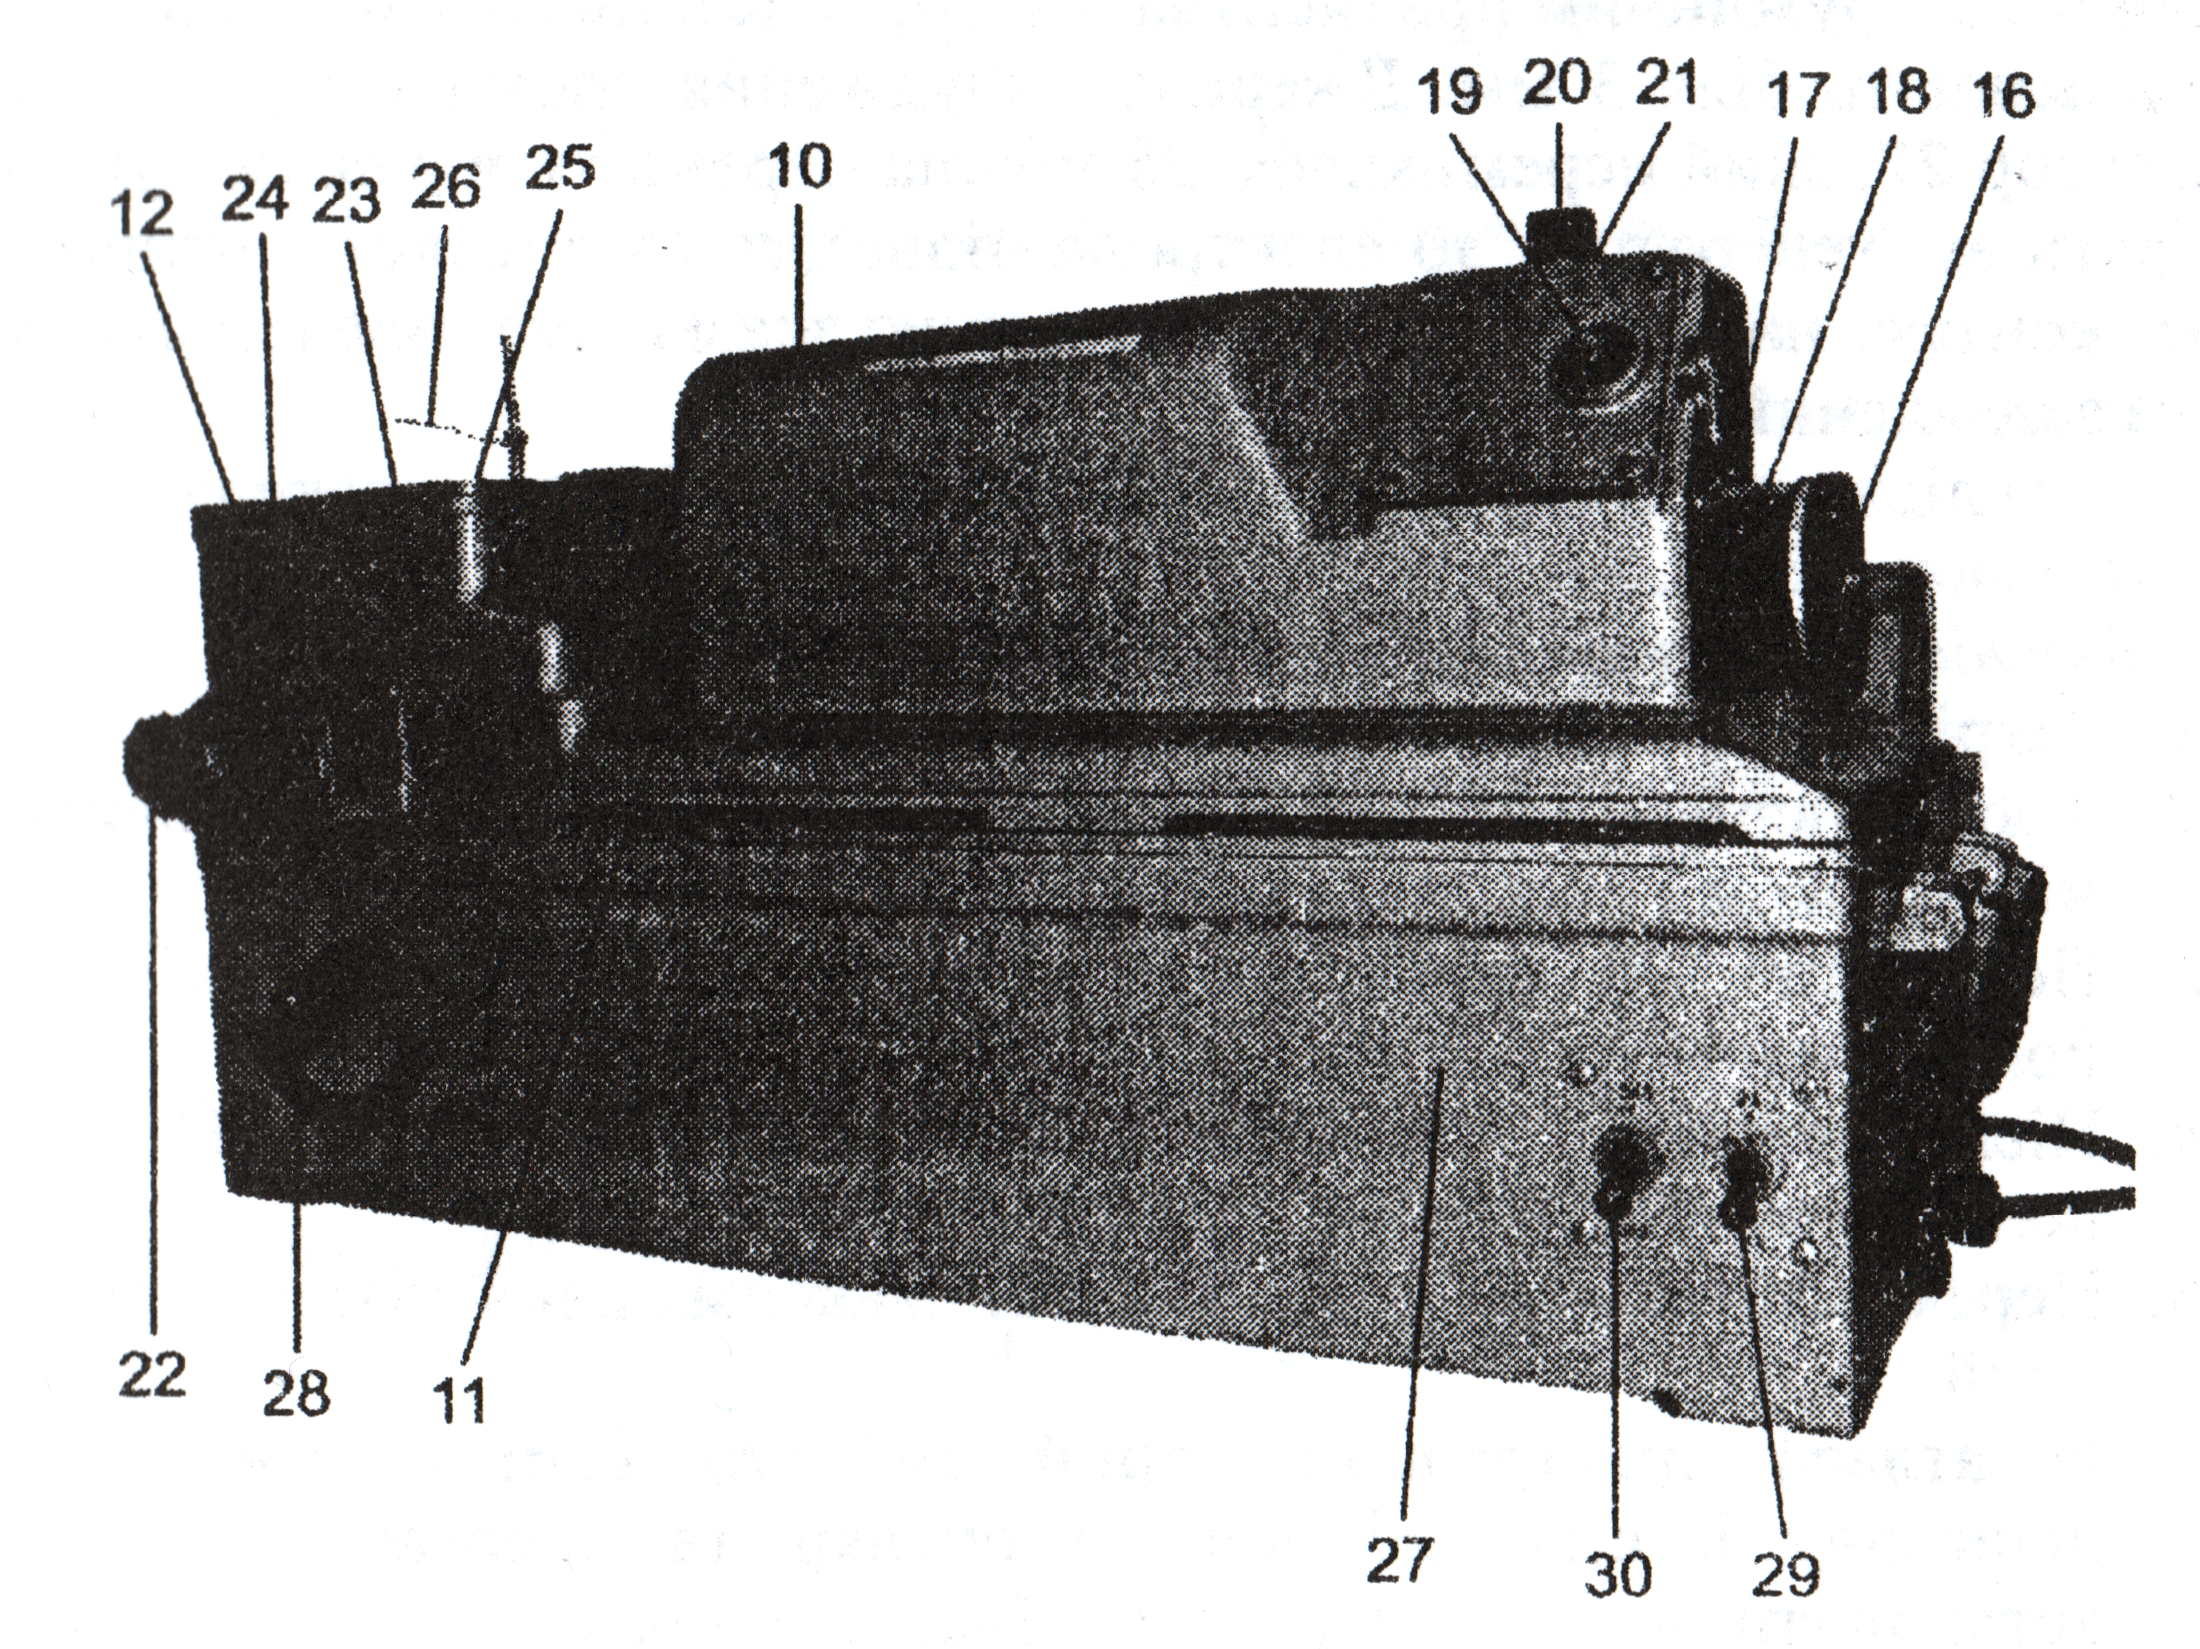
\includegraphics[width=80mm]{img_2}}
\caption{\source{}}
\label{img:2}
\end{figure}

Поворот призми здійснюється маховичком 16 (рис. \ref{img:2}), що з'єднаний з
барабаном, на якому нанесена рівномірна шкала 17 з ціною поділки 2 і шкала
18 з символами хімічних елементів. Символами позначені групи
спектральних ліній, що використовуються для аналізу сталі на відповідні
домішки. При суміщенні символу з відліковим штрихом барабана в полі зору
окуляра з'являється відповідна група ліній.

При обертанні маховичка 16 відбувається перефокусування об'єктиву,
а відповідно, і спектру, що спостерігається в полі зору окуляра, так як при
повороті призми повертається кулачок, що штовхає тубус об'єктива,
встановлюючи об'єктив у відповідне положення.

На кронштейні окулярної головки розташована прямокутна призма,
дзеркало, фотометричний клин зі шкалою і окуляр 19 в оправі.

Фотометричний клин розміщений в площині зображення спектра і
розташований вздовж спектральних ліній у вигляді вузької смуги в центрі
поля зору. Переміщення клину здійснюється маховичком і відраховується по
шкалі, що спостерігається в полі зору окуляра. У тих випадках, коли потрібно
працювати без фотометричного клина, слід маховичком привести в поле
зору діафрагму, що відповідає встановленому окуляру. Для цього необхідно
встановити крапку, що нанесена на маховичку, навпроти відповідного
позначення ($13.5^{x}$ або $20^{x}$) на шкалі 21.

На основі 11 розміщений також' тримач електродів, який можна
переміщувати по висоті маховичком 22 і в напрямку, перпендикулярному
оптичній вісі, - маховичком 23. Маховичком 24 можна обертати навколо
власної вісі дисковий електрод. Досліджуваний зразок закріплюють на
столику 25 пружинним притискувачем 26. Відстань між зразком і електродом
встановлюють біля 3 мм. Джерелом збудження спектра слугує спеціальний
генератор 27, який перемикачем 28 можна перевести в режим дуги або іскри.
Напруга від генератора до електрода підводиться високовольтним проводом
через контакт на кронштейні тримача, а до зразка, встановленого на столику,
через заземлений корпус приладу.

Досліджуваний зразок слід очистити від фарби, жужелиці, іржі тощо.
Зразком може бути, наприклад, свердло для металу.

%\begin{equation} \label{eq:Einstein}
%hv = A+\frac{m_{e}V_{max}^{2}}{2}
%\end{equation}



%\begin{table}[ht]
%\processtable{Спектральні характеристики деяких скляних світлофільтрів}
%{\begin{tabular}{|l|l|l|l|l|}\hline
%\thead{№} & 
%\thead{{\scriptsize Марка} \\ {\scriptsize світлофільтра}} & 
%\thead{{\scriptsize Товщина} \\ {\scriptsize скла, мм}} & 
%\thead{{\scriptsize Довжина хвилі} \\ {\scriptsize максимального} \\ {\scriptsize пропускання, м}} & 
%\thead{{\scriptsize Частота хвилі} \\ {\scriptsize максимального} \\ {\scriptsize пропускання, Гц}}\\\hline
%1 & КС-13 & 2,78 & $700*10^{-9}$ & $4.3*10^{14}$ \\\hline
%2 & OC-13 & 3,02 & $650*10^{-9}$ & $4.6*10^{14}$ \\\hline
%3 & ЖС-18 & 3,07 & $600*10^{-9}$ & $5.0*10^{14}$ \\\hline
%4 & 3C-1 & 1,00 & $540*10^{-9}$ & $506*10^{14}$ \\\hline
%5 & CC-2 & 1,00 & $390*10^{-9}$ & $7.7*10^{14}$ \\\hline
%6 & ФС-6 & 1,00 & $360*10^{-9}$ & $8.3*10^{14}$ \\\hline
%\end{tabular}}{}
%\end{table}

\newpage
\section{Послідовність виконання роботи}

\begin{enumerate}
	\item  Закріпити зразок на столику.
	\item Користуючись шаблоном та маховичками 22 і 23, встановити відстань
між зразком і дисковим електродом близько 3 мм.
	\item Перемикач 28 перевести в положення «Іскра», тумблер 29 - у
положення «2А».
	\item Після перевірки заземлення генератора, перемикач 30 перевести В
положення «Вкл».
	\item Переміщуючи окуляр 19, досягти максимальної чіткості спектральних
ліній.
	\item  Із атласа спектральних ліній вибрати картку певного видимого
діапазону і, спостерігаючи в окуляр та обертаючи маховичок 1б,
встановити в поле зору ту область спектра, яка відповідає картці
атласа.
	\item Зіставити спостережувані спектральні лінії з лініями картки і оцінити
	вміст елементів у досліджуваному зразку.
	\item Дії пунктів 6 і 7 повторити для інших спектральних областей.
	\item Експерименти провести у різних режимах роботи генератора.
\end{enumerate}


\begin{thebibliography}{}

\bibitem{1}
Кучерук І.М., Горбачук І.Т. Загальний курс фізики: Т.3.: Оптика.
Квантова фізика. -- К.: Техніка, 2006. - 518с., ст.200 - 203.

\bibitem{2}
Кучерук І.М, Дущенко В.П. Загальна фізика. Оптика. Квантова
фізика. - К.: Вища школа, 1991. - 463с., ст. 220 -224.

\bibitem{3}
Дущенко В.П. Фізичний практикум. - К.: Вища школа, 1984. --
256с., ст.207 - 211.

\bibitem{4}
Методична розробка до роботи.

\end{thebibliography}

\section{Завдання для самоконтролю}

\begin{enumerate}
	\item Які існують типи спектрів?
	\item Який внутрішній механізм випромінювання світла атомами
речовини?
	\item Які фізичні основи розкладання випромінювання світла в спектр?
	\item Що таке спектральна лінія? Від чого залежить її ширина?
	\item Чим відрізняються лінійчасті спектри випромінювання
і поглинання?
	\item У чому суть якісного і кількісного спектрального аналізу?
	\item Чим відрізняється абсорбційний аналіз від емісійного?
	\item Які домішки можна виявити у сплавах заліза?
	\item Які спектральні серії атому водню Вам відомі?
	\item Яка будова і принцип дії стилоскопа?
\end{enumerate}

\clearpage
\section{Тестові завдання для вхідного контролю}

\begin{enumerate}
	\item В основі спектрального аналізу знаходиться явище:
	\begin{enumerate}
		\item інтерференції;
		\item дифракції;
		\item дисперсії;
		\item поляризації.
	\end{enumerate}
	\item У даній роботі дослідження проводиться за допомогою:
	\begin{enumerate}
		\item спектроскопа;
		\item спектрографа;
		\item спектрометра;
		\item спектрофотометра.
	\end{enumerate}
	\item За допомогою стилоскопа СЛ-11А можна проводити дослідження в
областях (-і) спектра:
	\begin{enumerate}
		\item інфрачервоній;
		\item видимій;
		\item ультрафіолетвій;
		\item інфрачервоній, видимій, ультрафіолетвій.
	\end{enumerate}
	\item Аналіз у цій роботі проводиться на основі дослідження:
	\begin{enumerate}
		\item лінійчастого спектра емісії;
		\item лінійчастого спектра абсорбції;
		\item смугастого спектра поглинання;
		\item суцільного спектра випромінювання.
	\end{enumerate}
	\item Лінійчастий спектр поглинання дають:
	\begin{enumerate}
		\item атоми при їх нагріванні;
		\item молекули при їх збудженні;
		\item атоми при звичайних температурах;
		\item гази при високому тиску.
	\end{enumerate}
	\item При якісному спектральному аналізі наявність у речовині певних домішок
визначається:
	\begin{enumerate}
		\item за шириною спектральних ліній;
		\item за яскравістю спектральних ліній;
		\item за кількістю спектральних ліній;
		\item за допомогою спектральних атласів.
	\end{enumerate}
	\item За допомогою спектрального аналізу можна виявити наявність домішок,
концентрація яких не перевищує:
	\begin{enumerate}
		\item $10^{-6}\%$;
		\item $10^{-4}\%$;
		\item $10^{-2}\%$;
		\item $10^{-1}\%$.
	\end{enumerate}
	\item Диспергуюча система стилоскопа СЛ-11А складається 3:
	\begin{enumerate}
		\item однієї призми;
		\item двох призм;
		\item трьох призм;
		\item чотирьох призм.
	\end{enumerate}
\end{enumerate}

\newpage

\section{Тестові завдання для підсумкового контролю}

\begin{enumerate}
	\item Метою спектрального аналізу є:
	\begin{enumerate}
		\item визначення міжатомних відстаней у речовині;
		\item визначення складу речовини;
		\item вимірювання розмірів атомів та молекул речовини;
		\item вивчення випромінювальної здатності речовини.
	\end{enumerate}
	\item У даній роботі досліджується спектр:
	\begin{enumerate}
		\item емісійний;
		\item абсорбційний;
		\item комбінаційний;
		\item рентгенівський.
	\end{enumerate}
	\item У спектральних приладах основними елементами є:
	\begin{enumerate}
		\item щілини;
		\item лінзи;
		\item призми;
		\item фотопластинки.
	\end{enumerate}
	\item Стилоскоп СЛ-11А належить до:
	\begin{enumerate}
		\item спектрометрів;
		\item монохроматорів;
		\item спектрографів;
		\item спектроскопів.
	\end{enumerate}
	\item Лінійчатий спектр випромінювання можна одержати:
	\begin{enumerate}
		\item при нагріванні будь-якої речовини не залежно від її агрегатного стану;
		\item від нагрітих атомів;
		\item при нагріванні молекул;
		\item від нагрітих атомів при високому тиску.
	\end{enumerate}
	\item Оптичні елементи у стилоскопі СЛ-11А виготовлені із:
	\begin{enumerate}
		\item кварцу;
		\item скла;
		\item органічного скла;
		\item лужно-галоїдних монокристалів.
	\end{enumerate}
	\item Які з нижче перелічених характеристик оптичних систем притаманні
	спектральним приладам: 1) кутова дисперсія, 2) лінійна дисперсія,
3) збільшення, 4) оптична сила, 5) світлосила, 6) роздільна здатність,
7) відносний отвір?
	\begin{enumerate}
		\item всі сім; 
		\item перша, друга, п'ята та шоста;
		\item всі перелічені, крім третьої;
		\item третя, четверта та сьома.
	\end{enumerate}
	\item Кількість певної речовини у досліджуваному зразку на основі
спектрального аналізу можна оцінити за:
	\begin{enumerate}
		\item допомогою спеціальних таблиць і атласів;
		\item шириною спектральних ліній;
		\item кількістю спектральних ліній;
		\item інтенсивністю ліній.
	\end{enumerate}
	\item Кутовою дисперсією призми $D$ є:
	\begin{enumerate}
		\item $D = \frac{d \lambda}{d \phi}$;
		\item $D = d \lambda \cdot d \phi$;
		\item $D = \frac{d \phi}{d \lambda}$;
		\item $D = \frac{\phi}{d \phi}$.
	\end{enumerate}
\end{enumerate}

\end{document}

%\begin{table}[b]
%\processtable{Coefficients and remainders for distribution KK ($k = 0.05$,
%$v = 3$, $c_{1} = 1.5$, $c_{2} = 4.5$)}
%{\begin{tabular}{|l|l|l|}\hline
%$n$ & $a_{n}^{2}$ & $r_{k}(1)$\\\hline
%0 & 3.602576748428 & 1.493719547999\\\hline
%1 & 1.384791111989 & 0.108928436101\\\hline
%2 & 0.108600438794 & 0.000327997399\\\hline
%3 & 0.000275794597 & 0.000052202814\\\hline
%4 & 0.000027616892 & 0.000024585922\\\hline
%5 & 0.000018178621 & 0.000006407300\\\hline
%\end{tabular}}{}
%\end{table}
%
%So, the basic preamble and main body will be:
%\verb"\documentclass[twocolumn]{el-author}"\\
%\verb"\usepackage[...]{packages}"\\
%\verb"\date{12 December 2012}"\\
%\verb"\title{...}"\\
%\verb"\author{...}"\\
%\verb"\abstract{...}"\\
%\verb"\maketitle{...}"\\
%\verb"\begin{document}"\\
%\verb"..."\\
%\verb"\section{...}"\\
%\verb"..."\\
%\verb"\section{..}"\\
%\verb"..."\\
%\verb"\end{document}"